% LHC and ATLAS detectors

\section{ Large Hadron Collider}
The Large Hadron Collider (LHC) is the world's largest and most powerful particle accelerator, which became operational in 2008. It is located near the border of Switzerland and France at the European Organization for Nuclear Research (CERN) and was designed to collide proton beams at the center-of-mass energy of $14\tev$. This thesis analyzes the data collected throughout 2011, when the LHC operated at $7\tev$. In 2012, the LHC operated at $8\tev$, while $13-14\tev$ energies are planned for 2015 and beyond.

\begin{figure}[phtb]
  \begin{center}
    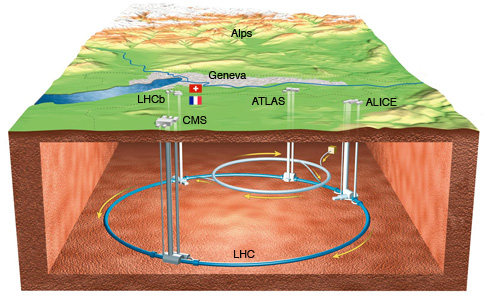
\includegraphics[width=0.7\textwidth]{det/fig/LHC_map}
    \caption{ The LHC tunnel and its four main experiments: ATLAS, ALICE, CMS, and LHCb.}
    \label{fig:det:tunnel}
  \end{center}
\end{figure}

The LHC lies in a 27-km tunnel buried about 170 meters underground (Fig.~\ref{fig:det:tunnel}). Four main experiments are located around the LHC ring. ATLAS and CMS are general-purpose experiments designed to perform precision measurements and discover the Higgs boson and new physics beyond the Standard Model. ALICE studies heavy ion collisions, while LHCb specializes in b-physics and forward measurements.

\subsection{ Beam Structure }
The collider tunnel hosts a super-conducting magnet system that supports two proton beams traveling in opposite directions around the circle. 1232 dipole magnets supply bending power, while 392 quadrupoles keep the beam focused~\cite{Brüning:782076}.

% http://www.lhc-closer.es/1/3/9/0
\begin{figure}[phtb]
  \begin{center}
        \subfigure[Protons colliding in bunches]{%
          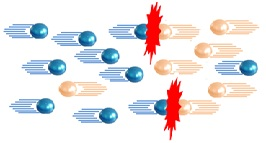
\includegraphics[width=0.44\textwidth]{det/fig/beam}
        } 
        \subfigure[Primary and pile-up interactions]{%
          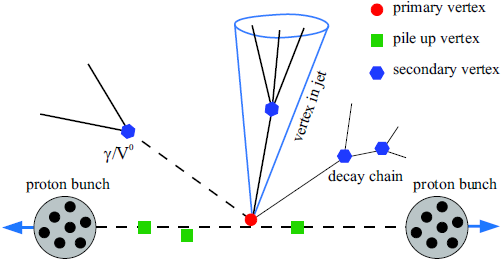
\includegraphics[width=0.44\textwidth]{det/fig/collision}
        }
 \caption{ Diagrams illustrating collision of proton bunches at the LHC.}
 \label{fig:det:bunches}
 \end{center}
\end{figure}

During a ``fill'', which happens approximately once a day, new protons are injected into the beam. They are organized into compact clusters called ``bunches'' that are spread around the circumference of the collider. The exact bunch structure is generally configurable and normally changes throughout the year, but the following are the prevailing conditions during 2011 data-taking~\cite{ATLAS-DAPR-2011-01-002}. The maximum number of bunch pairs in the tunnel at any given time (for clockwise and counterclockwise beams) is 1331. A typical bunch has $1.2 \cdot 10^{11}$ protons, and bunches meet every 50 ns. Despite a huge number of protons in the colliding bunches, each collision produces only about a dozen inelastic interactions. In an overwhelming majority of cases, only one of those interactions, called the ``primary'', produces interesting physics, while the others, called ``pileup'', end up depositing noise in the detector (Fig.~\ref{fig:det:bunches}).

\section{ The ATLAS Detector }

ATLAS (A Toroidal LHC Apparatus) is a complex machine that measures 25 meters in diameter and 46 meters in length, weighing nearly 7000 tonnes~\cite{Aad:2009wy}. It consists of a succession of particle detectors that surround the beam pipe and are centered on the nominal collision point (Fig.~\ref{fig:det:passage}). The innermost layers are instrumented with fine-grained tracking detectors submerged in a two-tesla solenoid field that bends charged particles in the plane transverse to the beam, providing a measurement of their momentum. Next, electromagnetic and hadronic calorimeters measure energy depositions from photons, electrons, and strongly-interacting particles, such as pions, protons and neutrons. Finally, the muon spectrometer, which provides a measurement of muon momentum, contains a variable toroidal magnetic field that bends charged particles in the longitudinal plane.

The detector is largely symmetric around the $\eta=0$ point. By convention, the $\eta<0$ and $\eta>0$ regions are called C-side and A-side, respectively.

\begin{figure}[phtb]
  \begin{center}
    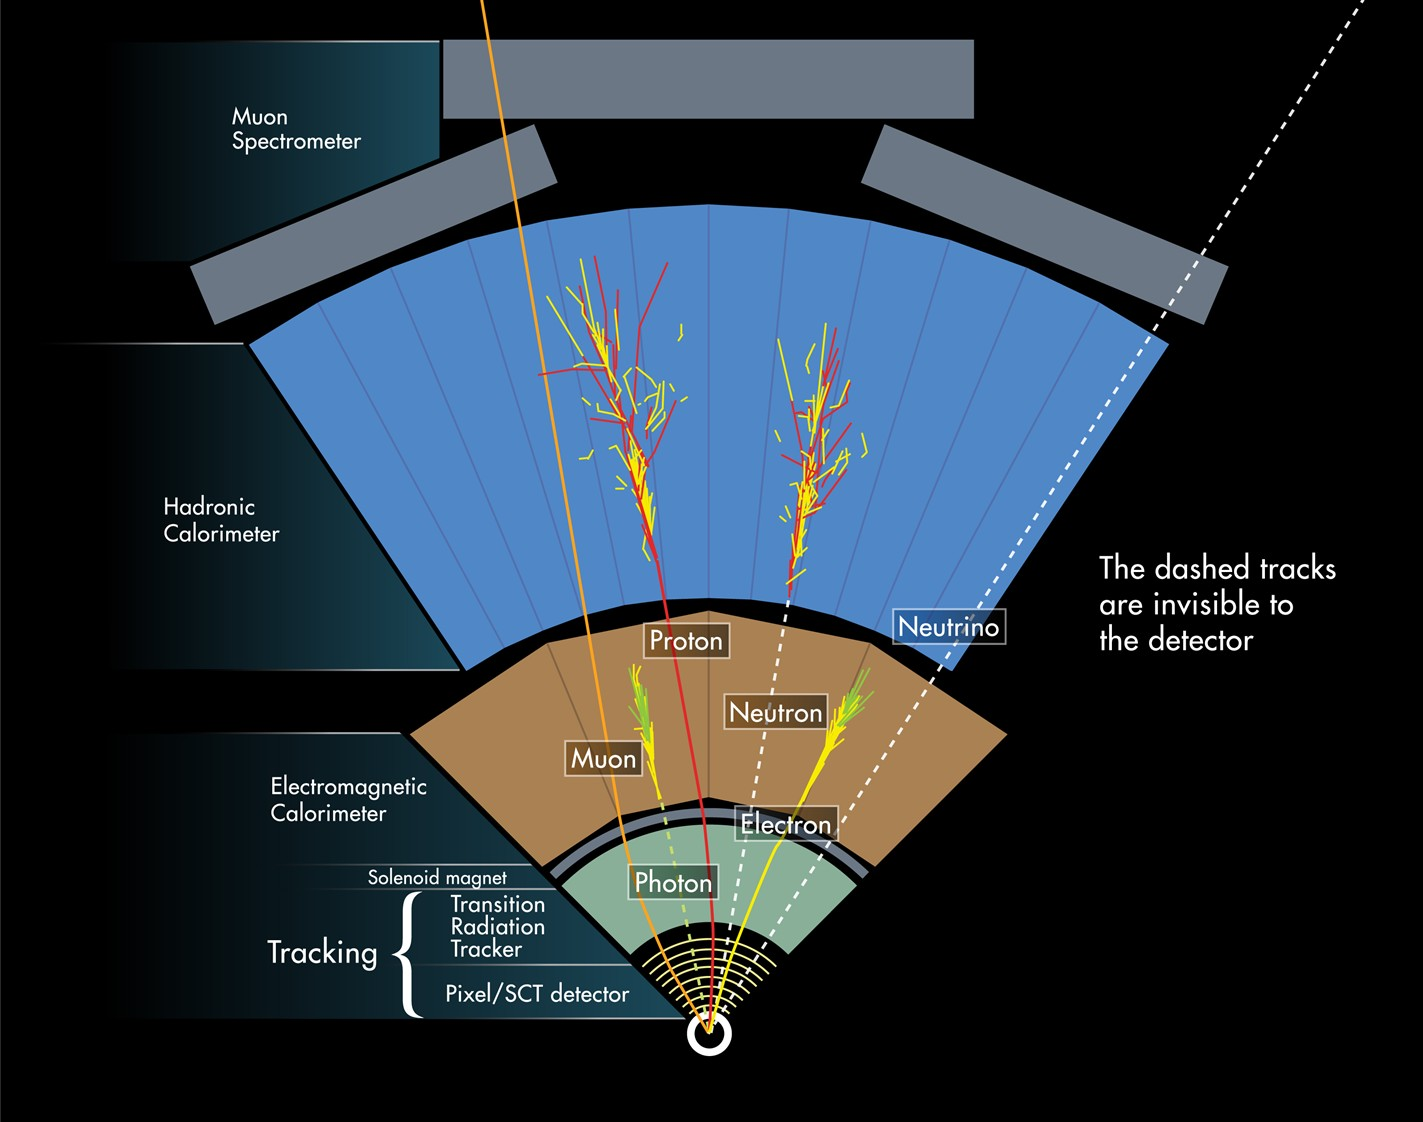
\includegraphics[width=0.80\textwidth]{det/fig/detection}
    \caption{ A diagram showing the ability of different ATLAS components to detect various particles produced in the collisions. }
    \label{fig:det:passage}
  \end{center}
\end{figure}

\subsection{ Inner Detector }
\label{chap:det:id}
The Inner Detector (ID) consists of the Pixel subsystem, Semiconductor Tracker (SCT), and Transition Radiation Tracker (TRT). These detectors play a crucial role in this analysis by measuring $\eta$, $p_{T}$, and other tracking parameters of muons from the \Wmn\ decay.

Fig.~\ref{fig:det:indet_side} shows a side view of the ID subsystems, which altogether span 6.2 meters in length and 2.1 meters in diameter. The region within approximately $|\eta|<1.1$ is called the ``Barrel'', reflecting the fact that the detectors in this region are shaped in barrel-like cylinders concentric around the beam pipe. The more forward region (larger $\eta$) is called the ``Endcap'' and is instrumented with disk-like structures with the sensitive layers positioned radially in the transverse plane.

\begin{figure}[phtb]
  \begin{center}
        \subfigure[Components of the Inner Detector]{%
          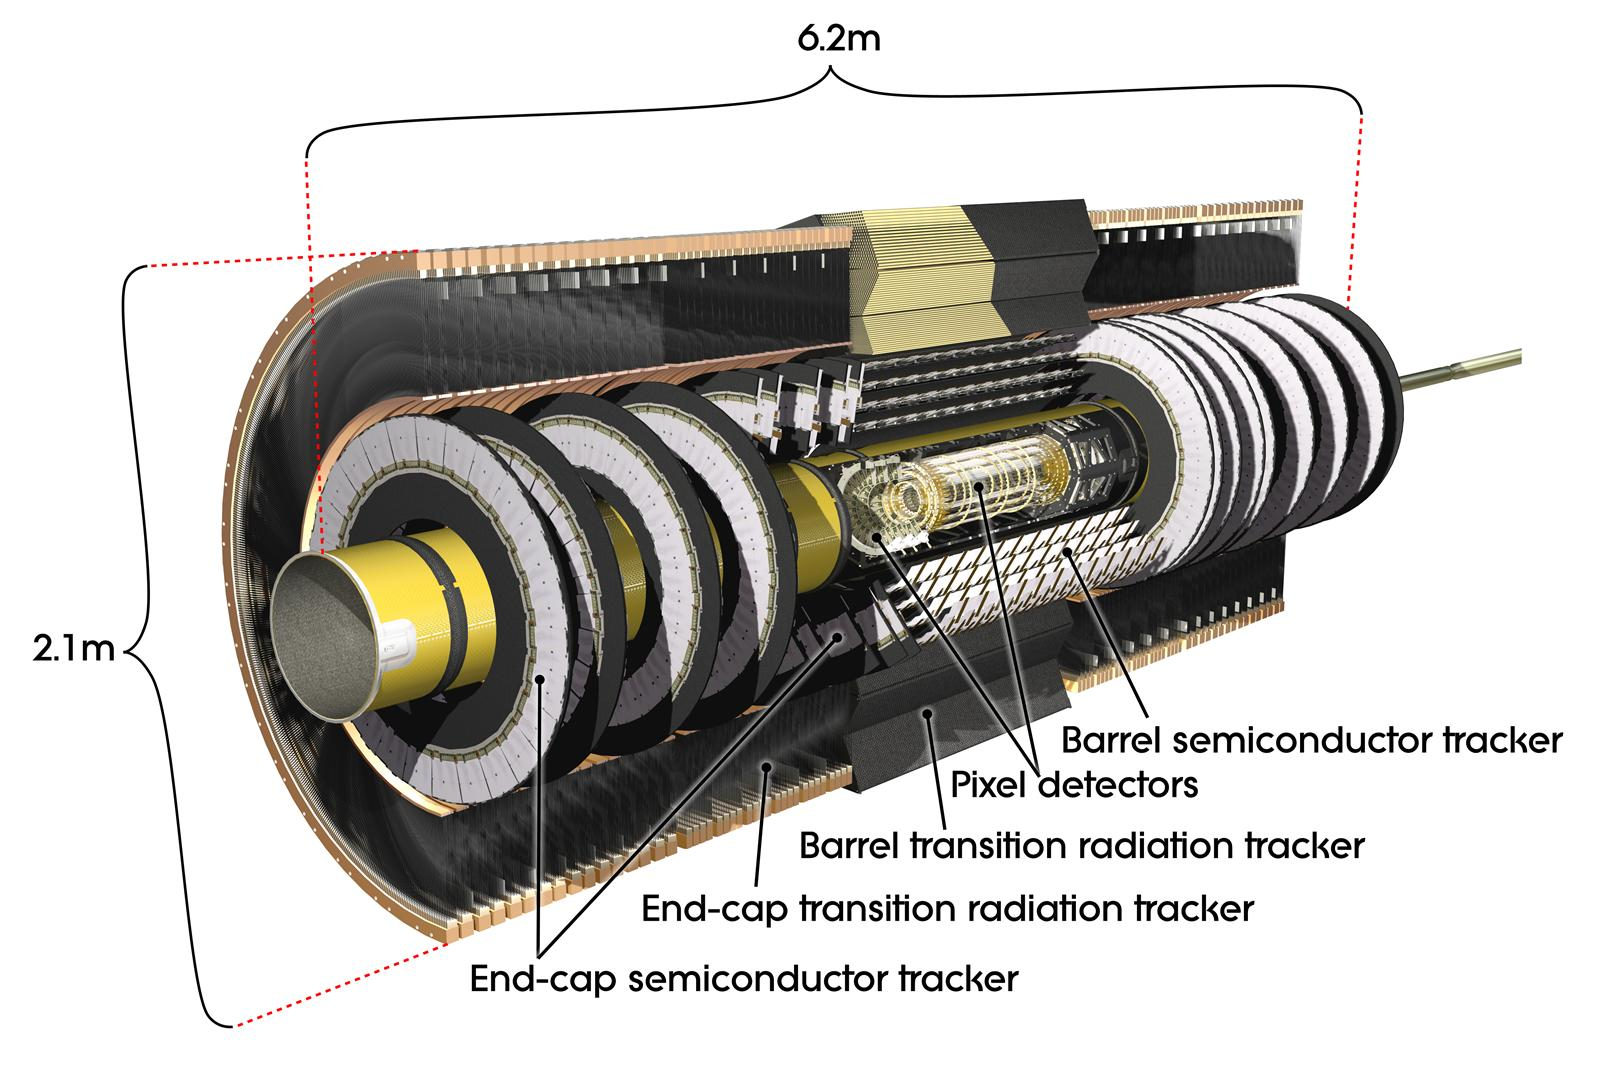
\includegraphics[width=0.8\textwidth]{det/fig/indet_side}
        }  \\
        \subfigure[Side view showing $\eta$ coverage]{%
          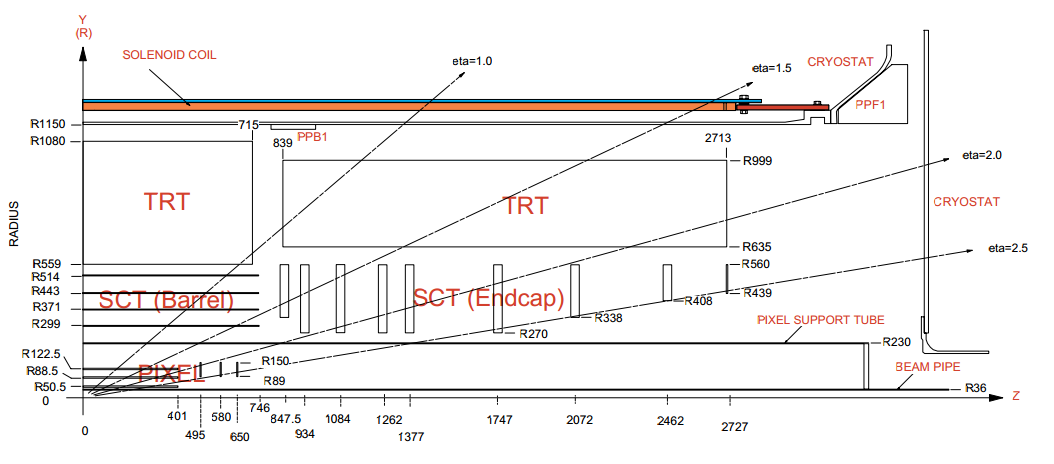
\includegraphics[width=0.8\textwidth]{det/fig/indet_etaview}
        }
 \caption{  Sub-components of the ATLAS Inner Detector and their $\eta$ coverage. }
 \label{fig:det:indet_side}
 \end{center}
\end{figure}

The Pixel detectors provide high-granularity tracking closest to the beam pipe (Fig.~\ref{fig:det:indet_xsec}). Each of the 1744 Pixel modules can be viewed as a two-dimensional sensor grid with $144$ measurement points along the $z$ axis and $328$ along the $R-\phi$ plane. Each sensor is $50$ x $400$ $\mu m^2$ and provides a time-over-threshold measurement of the energy deposited by the particles~\cite{1748-0221-3-07-P07007}. In total, the Pixel detector contains 80.4 million readout channels and is supported by a vast array of readout electronics. Pixel modules are arranged so that a typical track within the fiducial volume ($|\eta|<2.5$) crosses three detection layers.

The SCT detector is located outside of the Pixel system extending up to the radius of 65 centimeters. It consists of 4088 modules instrumented with silicon strips that provide a binary (on-off) readout. SCT modules have two measurement planes with 768 strips each: one plane with strips running parallel to the beam line and measuring hit positions in the $\phi$ direction, and another ``stereo'' plane offset by $40$ $mrad$ and providing information about $\eta$~\cite{1748-0221-3-10-P10006}. The strips are separated by about $80$ $\mu m$. In total, the SCT detector contains 6.3 million readout channels. SCT modules are arranged so that a typical track within the fiducial volume ($|\eta|<2.5$) crosses at least eight detection layers.

% on transition radiation: http://arxiv.org/pdf/hep-ex/0311058v1.pdf
The TRT detector consists of about 350,000 $4$ mm-diameter proportional straw tubes covering the region up to $|\eta|<2.0$. A typical track leaves 30 hits in the detector. The TRT extends to a radius of 1 meter, providing a long lever arm to measure the track parameters. Additionally, the TRT can detect transition radiation (photons emitted when a charged particle moves through an inhomogeneous medium), which is used to distinguish electrons from other minimum-ionizing particles, such as pions~\cite{1748-0221-3-02-P02013}.

\begin{figure}[phtb]
  \begin{center}
    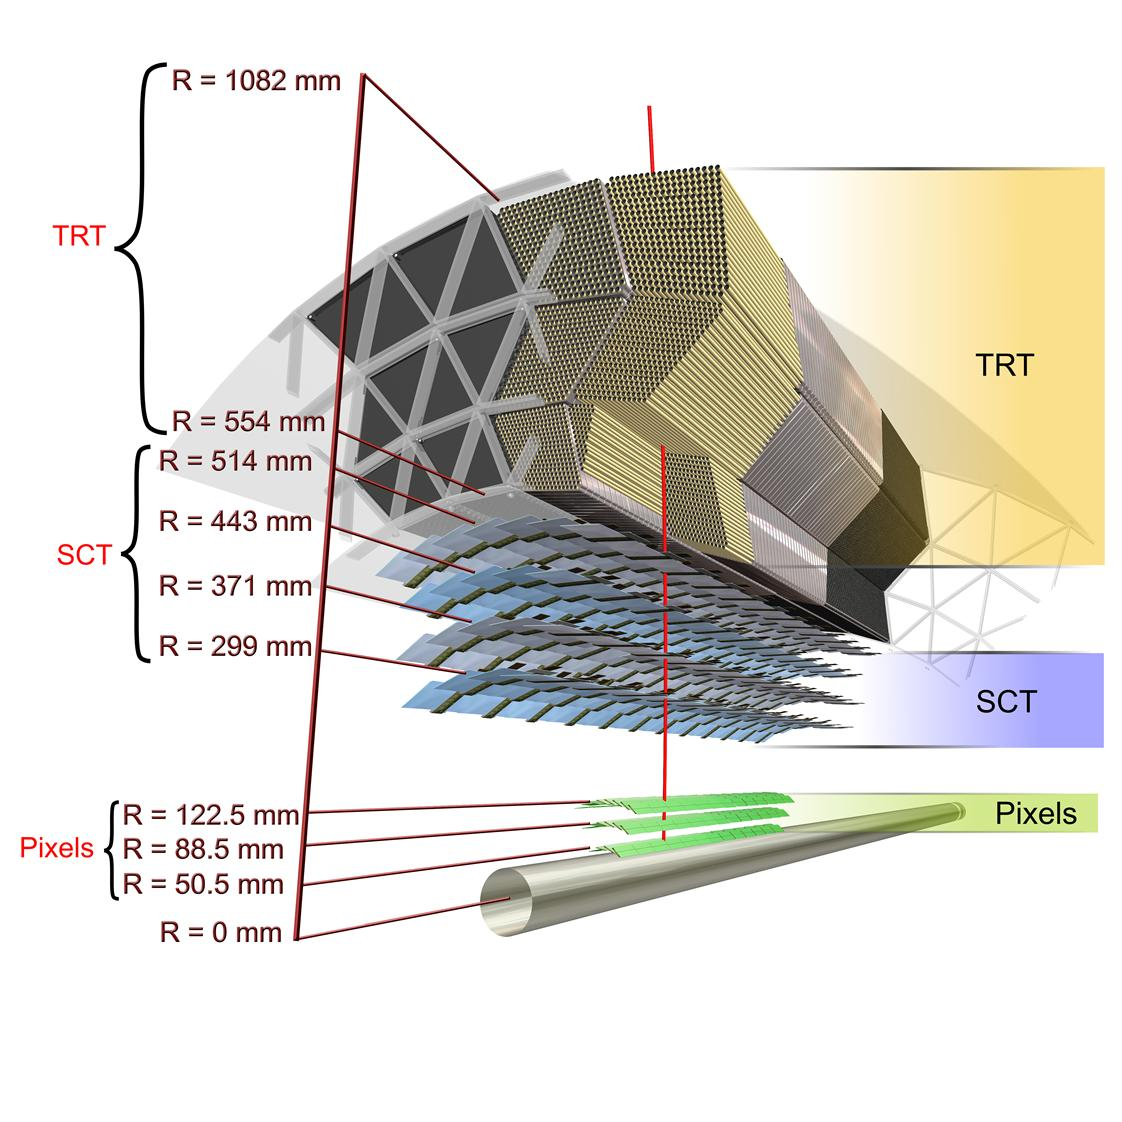
\includegraphics[width=0.70\textwidth]{det/fig/indet_xsec}
    \caption{ Cross-section view of the ATLAS Inner Detector, showing individual Pixel, SCT, and TRT modules. }
    \label{fig:det:indet_xsec}
  \end{center}
\end{figure}

\subsection{ Calorimeters }

Calorimeters are located outside of the Inner Detector solenoid magnet and measure the energy of the particles by absorbing them. The ATLAS calorimetry system consists of two parts: the electromagnetic calorimeter (EM) and the hadronic calorimeter (Fig.~\ref{fig:det:calo}). In the context of this analysis, calorimetry plays a crucial role by measuring the transverse energy imbalance used to identify neutrinos in \Wmn\ decays, which go through the detector unimpeded.

\begin{figure}[phtb]
  \begin{center}
    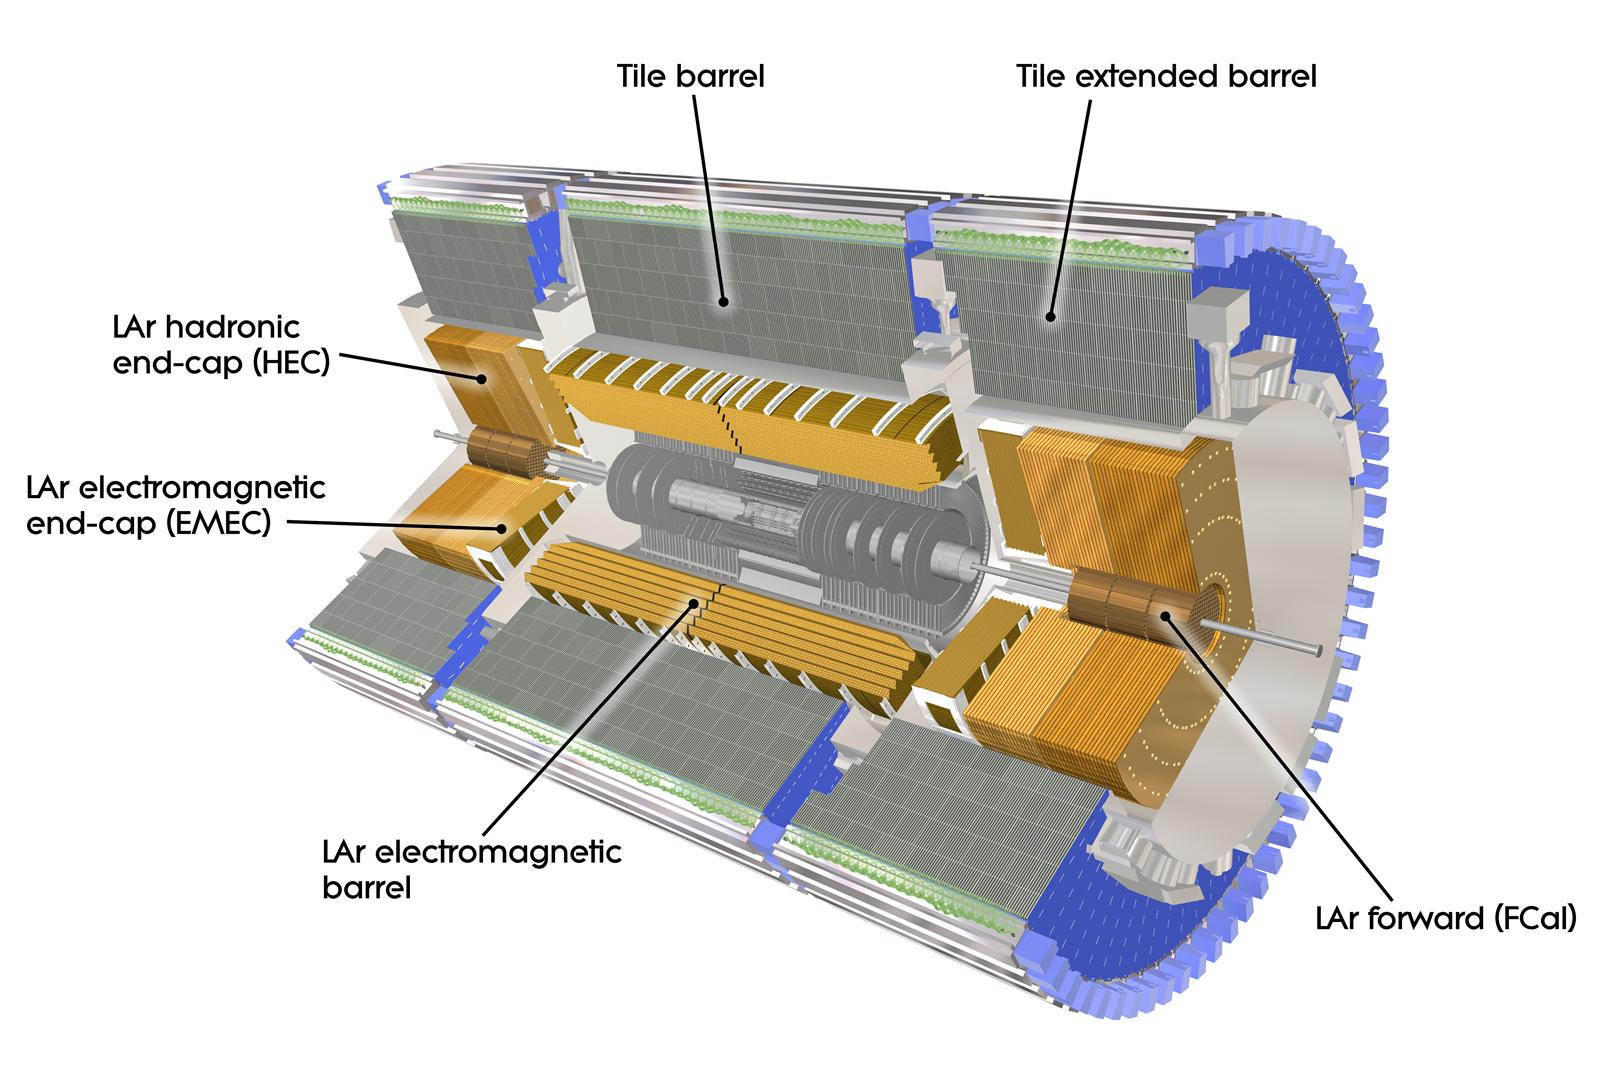
\includegraphics[width=0.80\textwidth]{det/fig/calo}
    \caption{ ATLAS calorimeter system. }
    \label{fig:det:calo}
  \end{center}
\end{figure}

The EM calorimeter, also called a LAr calorimeter, measures the energy of electromagnetically-interacting particles (photons and electrons) up to $|\eta|<3.2$. The active material is liquid argon (LAr), which is interspersed with accordion-shaped absorber plates made of lead or steel (Fig.~\ref{fig:det:accordion}). The total thickness of material is 20-22 radiation lengths, ensuring that the electrons and photos are stopped within the calorimeter~\cite{lar_tdr}. The calorimeter is segmented into 3 sampling layers and has a typical granularity of 0.025 radians in $\Delta\phi$ and $\Delta\eta$.

\begin{figure}[phtb]
  \begin{center}
    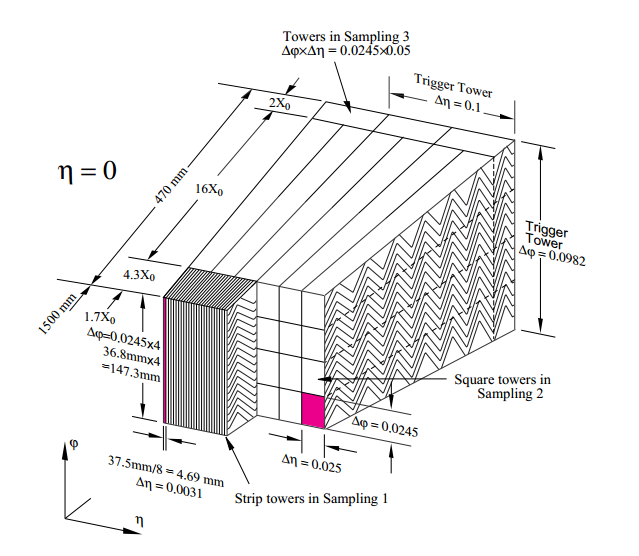
\includegraphics[width=0.70\textwidth]{det/fig/accordion}
    \caption{ Sketch of a section of the barrel EM calorimeter. }
    \label{fig:det:accordion}
  \end{center}
\end{figure}

The hadronic calorimeter measures the energy of strongly-interacting particles, such as pions. Its central portion, called Tile calorimeter, covers up to $|\eta|<1.7$ and uses steel as the absorber and scintillating tiles as the active medium (Fig.~\ref{fig:det:tile}). The tile calorimeter has a typical granularity of 0.1 radians in $\Delta\phi$ and 0.1 in $\Delta\eta$~\cite{tile_tdr} and is instrumental in reconstructing hadronic jets. The total thickness of the material exceeds 10 absorption lengths, which is sufficient to stop most hadrons within the calorimeter. Muons, however, are able to punch through after losing a few GeV in energy. The forward portions of the hadronic calorimeter extend $\eta$ coverage to 4.9 and, like the EM calorimeter, use the LAr technology, but with tungsten-copper absorbers.

\begin{figure}[phtb]
  \begin{center}
    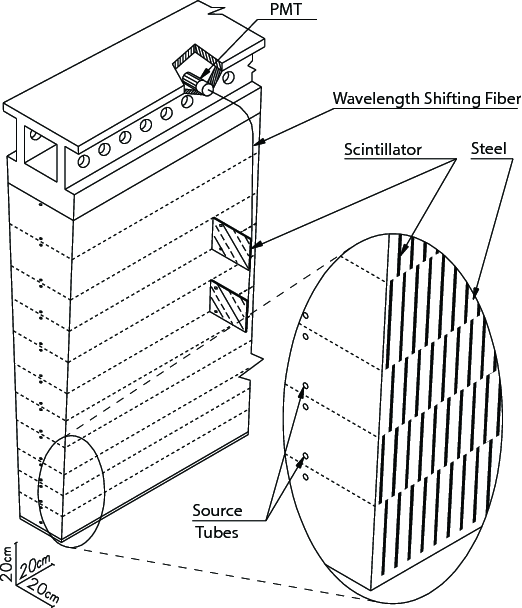
\includegraphics[width=0.50\textwidth]{det/fig/tile}
    \caption{ A wedge of the hadronic Tile calorimeter. }
    \label{fig:det:tile}
  \end{center}
\end{figure}

\subsection{ Muon Spectrometer }
\label{chap:det:ms}
The Inner Detector already measures the momentum of the muons. However, at sufficiently high $p_T$ (above 100 GeV), inner detector tracks look like straight lines, making it difficult to determine the charge (direction of bending) and the precise value of the momentum. The Muon Spectrometer mitigates these deficiencies by providing a much larger lever arm to measure the bending in the toroidal magnetic field. Because the muon spectrometer is placed after the calorimeters, it does not see the electrons or pions and can thus identify the charged particles it sees as muons. To ensure high-quality muon reconstruction, this analysis combines the measurements from the Inner Detector and Muon Spectrometer.

The Muon Spectrometer covers the area up to $|\eta|<2.7$ and consists of about 1300 chambers that go all the way to the outer radius of the ATLAS detector~\cite{muon_tdr}. As seen in Fig.~\ref{fig:det:muons}, a typical muon passes through 3 chambers. Four technologies are used in the muon system. Monitored Drift Tubes (MDT) do tracking in the Barrel while Cathode Strip Chambers (CSC) do the same in the Endcaps. For triggering, Resistive Plate Chambers (RPC) are used in the Barrel and Thin Gap Chambers (TGC) in the endcap. Trigger coverage is generally limited to $|\eta|<2.4$.

\begin{figure}[phtb]
  \begin{center}
        \subfigure[3-dimensional view]{%
          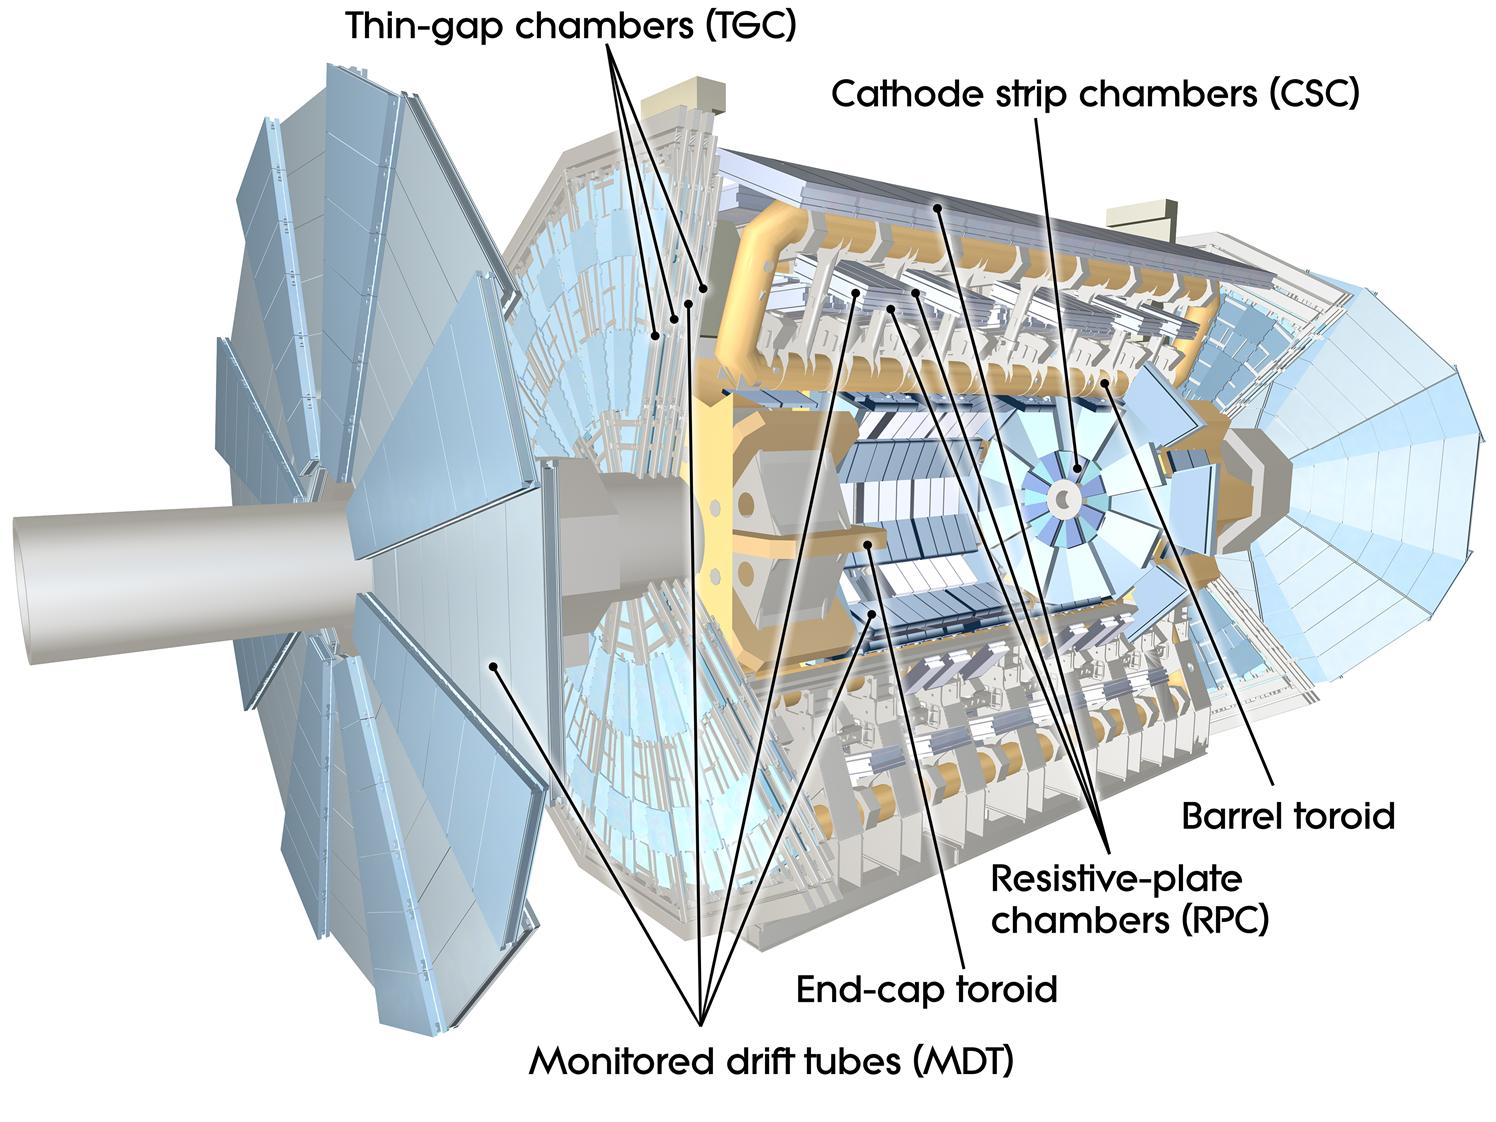
\includegraphics[width=0.7\textwidth]{det/fig/muons}
        }  \\
        \subfigure[Side view]{%
          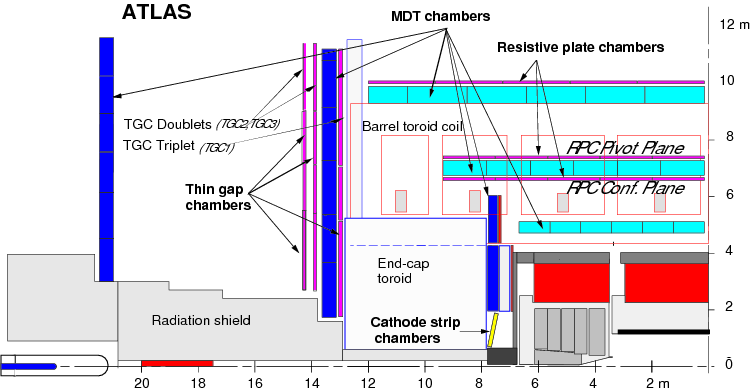
\includegraphics[width=0.8\textwidth]{det/fig/muonside}
        }
 \caption{ A sketch of the main components of the Muon Spectrometer. }
 \label{fig:det:muons}
 \end{center}
\end{figure}

\subsection{ Trigger and Data Acquisition }
\label{sec:det:trigger}
In 2011, the LHC collided proton bunches every 50 ns. Only a tiny fraction of these collisions can be stored for subsequent analysis, and immense real-time data reduction is needed that can select interesting physics while discarding un-eventful collisions. The ATLAS experiment employs a sophisticated three-level trigger system to achieve these goals~\cite{Jenni:616089}. Level-1 selection is performed in dedicated hardware that uses coarse-granularity information from calorimeters and muon spectrometers to apply cuts to a variety of objects, such as jets, muons, electromagnetic clusters, and missing energy. Level-2 and Event Filter, collectively known as High Level Triggers (HLT), are effectively large computer farms designed to refine the selection. Level-2 does limited reconstruction (including tracking) inside Regions of Interest (ROI) identified by the Level-1 trigger. Event Filter performs full-event reconstruction with near-offline quality. The events passing Event Filter are saved on disk.

As Fig.~\ref{fig:det:trigger} shows, the trigger system reduces event rate from 40 MHz down to 200 Hz - a 5-order of magnitude reduction.

\begin{figure}[phtb]
  \begin{center}
    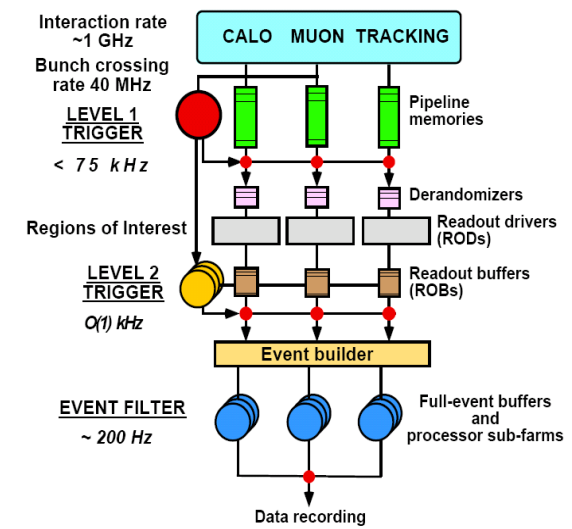
\includegraphics[width=0.60\textwidth]{det/fig/trigger}
    \caption{ The ATLAS trigger system. }
    \label{fig:det:trigger}
  \end{center}
\end{figure}


\subsection{ Computing }
% http://cds.cern.ch/record/840543/files/lhcc-2005-024.pdf

All data collected by ATLAS is initially stored at a central facility at CERN called Tier-0 and subsequently distributed to national Tier-1 centers. The US Tier-1 facility is located at the Brookhaven National Laboratory (BNL). Portions of the data are further replicated to regional Tier-2 facilities, one of which - the Midwest Tier-2 - is located at the University of Chicago. Altogether, the LHC Computing Grid consists of about 170 computing centers around the world, which provide over 200,000 CPUs and hundreds of petabytes of storage for data and Monte-Carlo processing~\cite{Eck:840543,citeulike:8657322}.

All data and Monte-Carlo datasets used in this analysis amount to about 500 terabytes in size. A data reduction algorithm running on the cloud converts these datasets to a more manageable set of ntuples requiring 5 terabytes of storage. These ntuples are stored at the Midwest Tier-2 facility and analyzed with about 1000 CPUs available at the university.

